\documentclass[14pt]{beamer}
\usepackage{hyperref}
\usetheme{boxes}
\usepackage{color}
\usecolortheme{dove}
\usepackage{mathptmx}

\title{Backend Infrastructure}
\subtitle{Presented to Moringa School}
\author{Evan Klitzke}
\date{January 17, 2018}

\begin{document}

\begin{frame}
  \titlepage
\end{frame}

\AtBeginSection[]
{
  \begin{frame}[plain]{Outline}
    \tableofcontents[currentsection]
  \end{frame}
}

\begin{frame}
\frametitle{Outline}
  \tableofcontents
\end{frame}

\section{My Background}

\begin{frame}{About Me}
  I am a software engineer based out of San Francisco. I previously worked at
  Google and Uber, now I'm traveling, hacking on crypto stuff, and figuring out
  what's next.
  \newline
  \newline
  I spent most of 2017 working on different crypto projects. In February I'll be
  participating in the \href{https://hackerresidency.com}{Chaincode Residency}
  program in NYC to work on Bitcoin Core.
\end{frame}

\begin{frame}{How I Got Into Programming}
  I read this book when I was in high school, and thought it was the coolest
  thing ever:
  \newline
  \newline
  \makebox[\textwidth]{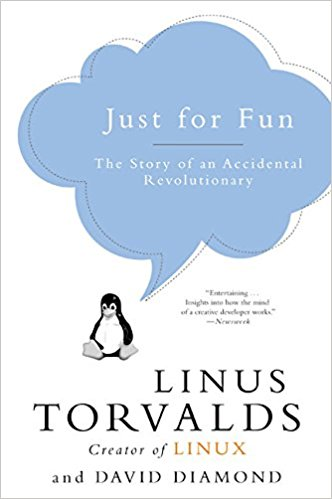
\includegraphics[scale=0.30]{linux.jpg}}
\end{frame}

\begin{frame}{Linux \& Open Source}
  The story of Linux is amazing---a college student in Finland wrote an
  operating system kernel all by himself.
  \newline
  \newline
  Linux is now the most popular OS in the world. It runs every Android phone in
  the world, and the vast majority of the world's servers. Every single
  supercomputer in the top 500 runs Linux.
\end{frame}

\begin{frame}{My First Open Source OS}
  \makebox[\textwidth]{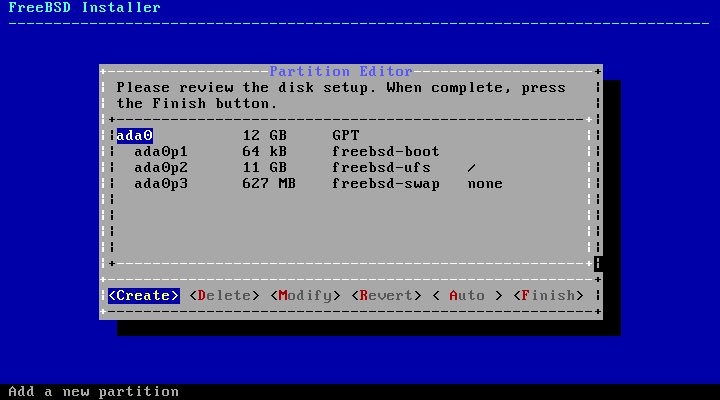
\includegraphics[scale=0.60]{bsd-installer.png}}
\end{frame}

\begin{frame}{I Nuked The Family Computer}
  I spent two days downloading the installer from an FTP site. My download
  failed because the FTP client I was using was set to text mode.
  \newline
  \newline
  After redownloading, I nuked the hard drive on my family computer and wasn't
  allowed to use Linux (or BSD) until I went to college.
\end{frame}

\begin{frame}{My First Unix Book}
  I went to college to study physics, and immediately picked this book up:
  \newline
  \newline
  \makebox[\textwidth]{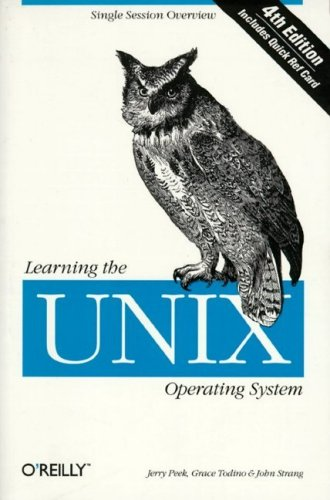
\includegraphics[scale=0.30]{oreilly.jpg}}
\end{frame}

\begin{frame}{Learning Unix/Linux}
  I installed Linux on my college laptop, and got obsessed. I thought it was the
  coolest thing. I was failing my classes but learning a lot about Linux.
  \newline
  \newline
  Since I was failing my classes I thought I was going to drop out, so I emailed
  a local LUG (Linux User's Group) and got an internship.
\end{frame}

\section{Yelp}

\begin{frame}{Yelp}
  This led to a job at a local startup from SF called Yelp.
  \newline
  \newline
  I was supposed to admin their servers, but they let me try out coding and I
  was pretty good at it.
\end{frame}

\begin{frame}{Yelp Hypergrowth}
  Yelp was growing really fast, and they couldn't keep up with the traffic. When
  Google would index the site, Yelp would go down.
  \newline
  \newline
  My boss asked me to fix it, which mostly involved optimizing SQL queries. I
  had no idea what I was doing, but I figured it out.
\end{frame}

\begin{frame}{Database Scaling}
  Databases are the limiting factor for scaling at most web companies.
  \newline
  \newline
  Databases are a big, central point of failure. They're hard to scale. If
  you're really good at optimizing database queries, you're worth your weight in
  gold.
\end{frame}

\begin{frame}{Database Replication}
  \makebox[\textwidth]{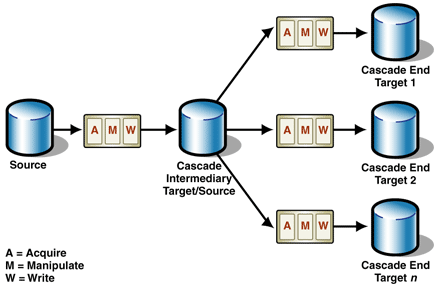
\includegraphics[scale=0.60]{replication.png}}
\end{frame}

\begin{frame}{Indexes}
  The key to optimizing database queries is understanding how B-trees and
  compound indexes work.
  \newline
  \newline
  FIXME
\end{frame}

\begin{frame}{Caching}
  The other trick for scaling databases is to add caching. Yelp used something
  called Memcached, another popular alternative widely used today is called
  Redis.
  \newline
  \newline
  The caching layer can do key-value lookups for data directly in memory,
  bypassing the disk.
\end{frame}

\begin{frame}{LAMP}
  Yelp was built with the following technology:
  \begin{itemize}
  \item Linux
  \item Apache
  \item MySQL
  \item Python
  \end{itemize}
  This stack is so popular it has its own acronym, LAMP.
\end{frame}

\begin{frame}{Multi-Datacenter Replication}
  My biggest project at Yelp was moving the company to a multi-datacenter setup.
  \newline
  \newline
  This is really difficult to do in a site that depends heavily on caching, due
  to stale reads.
\end{frame}

\section{Google}

\begin{frame}{Google}
  Eventually I went to this ad company called Google.
  \newline
  \newline
  It was pretty boring, I didn't even last there a year.
\end{frame}

\section{Uber}

\begin{frame}{Uber}
  Next up was this little (at the time) cab company called Uber.
  \newline
  \newline
  Uber was also using Python and MySQL. Some of the details were different, but
  overall the architecture was pretty similar to Yelp.
  \newline
  \newline
  The technology details differ from company to company, but the most important
  stuff is all the same.
\end{frame}

\begin{frame}{MySQL to Postgres}
  My first big project at Uber was moving them from MySQL to PostgreSQL, another
  relational database.
  \newline
  \newline
  This was a huge disaster, and it made things go from bad to worse. An
  important lesson here: make decisions based on technology, not hype!
\end{frame}

\begin{frame}{Connection Scalability}
  The main limitation that Postgres has is related to connection scalability and
  concurrency. This can't be fixed with indexes.
  \newline
  \newline
  I spent a year optimizing idle transactions.
\end{frame}

\begin{frame}{Schemaless}
  Eventually we decided that we needed to ditch Postgres.
  \newline
  \newline
  I helped design and implement a sharded key-value database storage layer built
  on MySQL.
\end{frame}

\begin{frame}{Python Profiling}
  Later I moved to a team that had the goal of optimizing all of the Python code
  at the company.
  \newline
  \newline
  I really wanted to use flame graphs, but there weren't any good Python
  profilers that could generate them. So I wrote one.
\end{frame}

\begin{frame}{Pyflame}
  Demos here.
\end{frame}

\section{Q{\&}A}

\begin{frame}{Slides and Contact Info}
  You can download the slides for this talk at:
  \textbf{\href{https://eklitzke.org/nairobi-moringa.pdf}{eklitzke.org/nairobi-moringa.pdf}}
  \newline
  \newline
  The source code for these slides can be found at:
  \href{https://github.com/eklitzke/nairobi-moringa}{github.com/eklitzke/nairobi-moringa}
  \newline
  \newline
  How to reach me in the future:
  \newline
  \newline
  \begin{tabular}{r | l}
    Email & \href{mailto:evan@eklitzke.org}{evan@eklitzke.org} \\
    Web & \href{https://eklitzke.org}{eklitzke.org} \\
    Twitter & \href{https://twitter.com/eklitzke}{@eklitzke} \\
  \end{tabular}
\end{frame}


\end{document}
